\chapter{Solución Propuesta}
\label{chap:proposal}

Un componente importante en la composición de imágenes realistas es la iluminación. Para el cálculo de iluminación directa bajo el pipeline de renderizado estándar ya se tienen décadas de estudio y distintas técnicas que permiten tiempos de renderizado muy cortos en hardware moderno. En contraste el cálculo de iluminación indirecta sigue siendo una tarea computacionalmente compleja. 

Para el cálculo de iluminación indirecta existen varios procedimientos muchos de estos inspirados en los ya explicados en la sección \ref{sub:render_eq_procedures}. Sin embargo estos no están pensados para renderizado en tiempo real. En la sección \ref{sec:interactive_gi_takes} examinamos algunas aproximaciones para el cálculo de iluminación indirecta en tiempo real, estas técnicas explotan ciertas características de hardware o recursos del pipeline de renderizado.

Parte de nuestra implementación para el cálculo de iluminación global en tiempo real está basada en el trabajo de Crassin et al. en 2011 \cite{CNSGE11b}. Este trabajo ya fue examinado en la sección \ref{sub:voxel_cone_tracing_orig}. La técnica fue escogida porque además de reflexión difusa también permite el cálculo de superficies lustrosas con reflexión especular a diferencia de otras técnicas como \ac{CLPV} que solo permiten reflexión difusa. Una ventaja de esta aproximación es que los valores de radiancia ya se encuentran almacenados sobre una representación con vóxeles. Esto acelera el cálculo de luz incidente bajo el esquema de integración Monte Carlo visto en la sección \ref{subsec:monte_carlo_raytracing}, en este caso los conos permiten realizar una cruda aproximación de un grupo de rayos. Además de esto el algoritmo puede ser usado en escenas totalmente dinámicas.

\section{Voxelización} % (fold)
\label{sec:voxelizacion}
El trazado de conos contra geometría poligonal compleja es costoso. Encontrar los puntos de intersección entre un cono y un polígono es mucho más complejo que intersecciones rayo-polígono, además de esto un solo cono podría intersectar muchos polígonos.

Para simplificar el trazado de conos se utiliza una discretización de la escena en forma de vóxeles. Esta representación puede ser filtrada a niveles más bajos de detalle (ver Figura \ref{fig:voxelization_details}). Esto nos permite aproximar el efecto de extensión sobre la apertura del cono utilizando cada vez un nivel de detalle más bajo a través del recorrido del mismo.

\begin{figure}[H]
	\centering
	\begin{subfigure}[b]{.32\linewidth}
		\centering
		\captionsetup{justification=centering}
		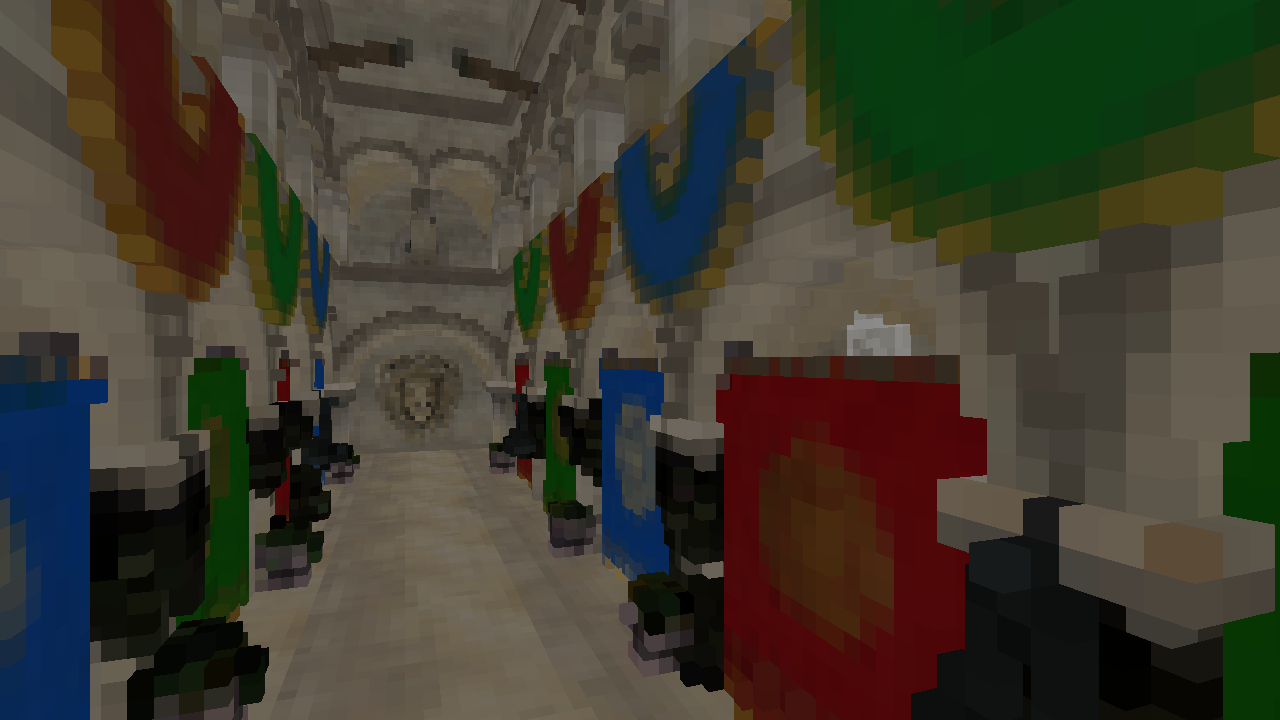
\includegraphics[width=\linewidth]{media/finals/albedo_v256.png}
	\end{subfigure}%
	\hspace{0.01\textwidth}
	\begin{subfigure}[b]{.32\linewidth}
		\centering
		\captionsetup{justification=centering}
		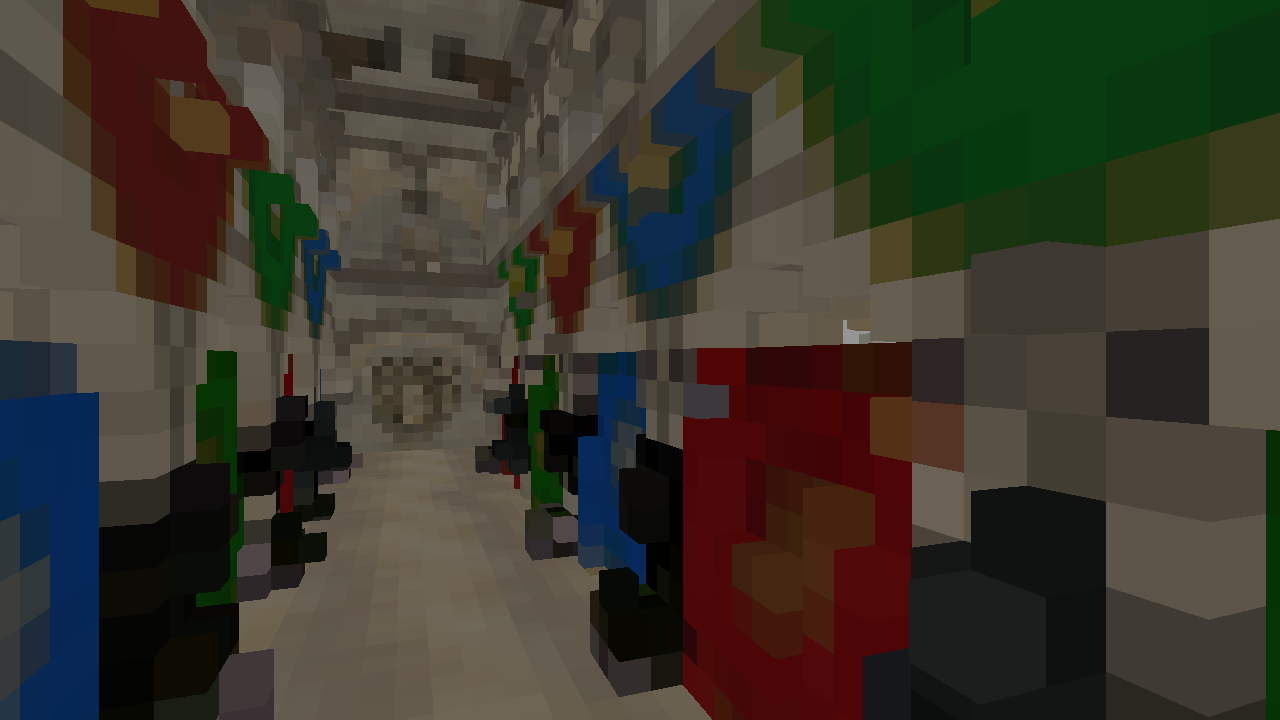
\includegraphics[width=\linewidth]{media/finals/albedo_v128.png}
	\end{subfigure}%
	\hspace{0.01\textwidth}
	\begin{subfigure}[b]{.32\linewidth}
		\centering
		\captionsetup{justification=centering}
		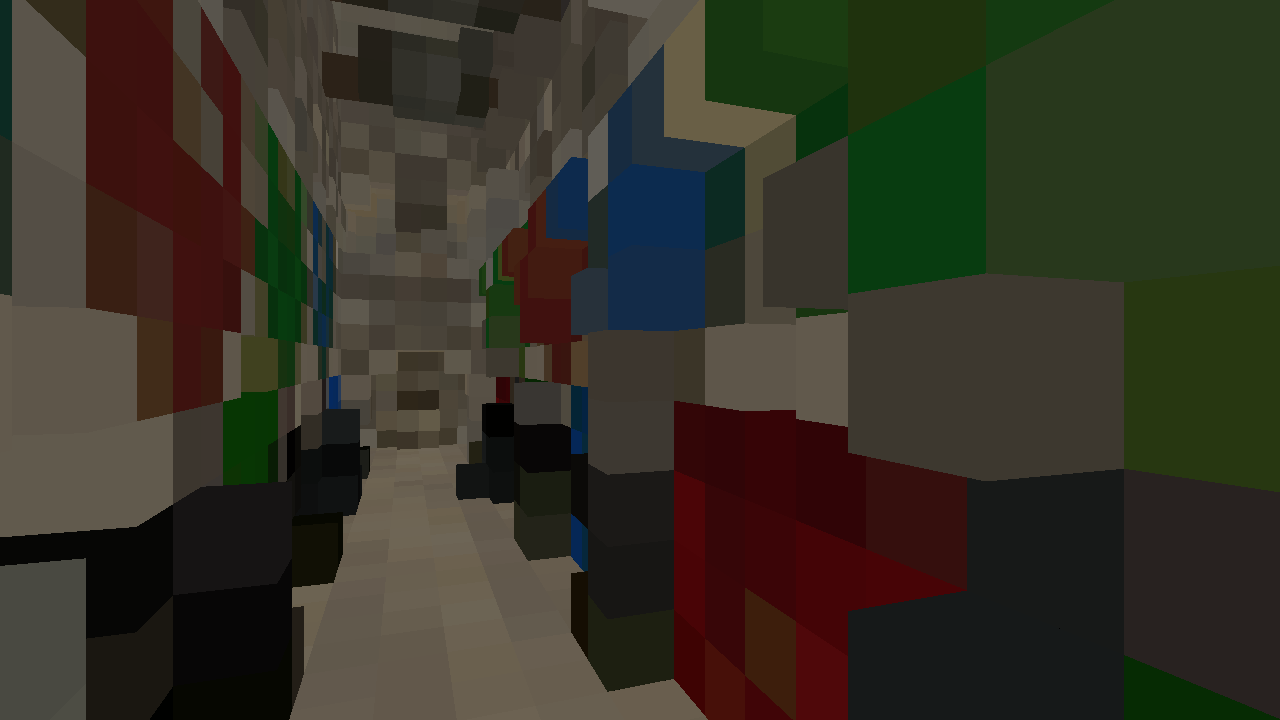
\includegraphics[width=\linewidth]{media/finals/albedo_v64.png}
	\end{subfigure}%
	\caption{Distintos niveles de detalle de una escena voxelizada.}
	\label{fig:voxelization_details}
\end{figure}

Para las partes dinámicas de la escena este proceso de voxelización debe ser realizado cada vez que sucede algún cambio sobre cualquier superficie que pertenece a un objeto dinámico. Por esta razón se requiere un algoritmo de voxelización de alto rendimiento para mantener tiempos interactivos.

\subsection{Voxelización Conservativa} % (fold)
\label{sub:voxelizacion_conservativa}
Nuestra implementación realiza voxelización conservativa de geometría de alto rendimiento utilizando la \ac{GPU} y explotando características del pipeline de renderizado con OpenGL. Para esto se implementó el algoritmo de voxelización utilizando rasterización en hardware explicado en el libro \emph{OpenGL Insights} por Cyril Crassin y Simon Green en \emph{Octree-Based Sparse
Voxelization Using the GPU
Hardware Rasterizer} \cite{CozziRiccio12}. Este algoritmo está basado en el trabajo de Zhang et al. en 2007 \cite{zhang2007conservative} para la voxelización conservativa utilizando la \ac{GPU} y el trabajo de Hasselgren et al. en 2005 \cite{hasselgren2005conservative} sobre rasterización conservativa. En la Figura \ref{fig:vox_pipeline} se puede observar la arquitectura descrita en \emph{Octree-Based Sparse Voxelization Using the GPU Hardware Rasterizer} para el proceso de voxelización. 

Para maximizar el área de rasterización la idea es proyectar cada triángulo utilizando proyección ortogonal por cada eje direccional. El eje dominante es escogido según el vector normal del plano definido por los vértices del triángulo.

\begin{figure}[H]
	\centering
	\captionsetup{justification=centering}
	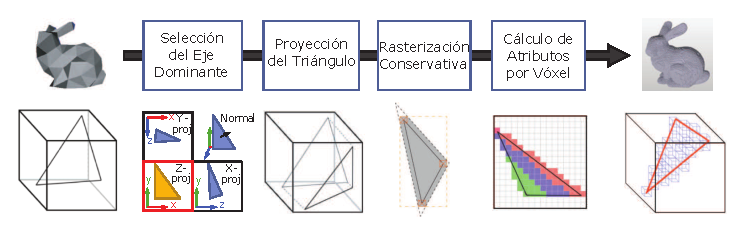
\includegraphics[width=\linewidth]{media/voxelization_pipeline.eps}
	\caption{Descripción del pipeline de voxelización \cite{CozziRiccio12}.}
	\label{fig:vox_pipeline}
\end{figure}
 
Por cada triángulo proyectado es necesario generar un polígono delimitante un poco más grande que el triángulo para garantizar la voxelización conservativa. Este polígono debe permitir que por cualquier triángulo proyectado tocando un píxel este va obligatoriamente a tocar el centro de este píxel, por tanto el pipeline de rasterización generara fragmentos para este triángulo. El polígono se genera expandiendo cada vértice del triángulo hacia afuera utilizando el procesador de geometría o \emph{geometry shader}. El polígono delimitante no sobreestima la cobertura del triángulo por tanto este no tiene forma de triángulo (ver Figura \ref{fig:expanded_bbpolygon}). Los fragmentos excedentes de este polígono son descartados en el \emph{fragment shader} utilizando una región delimitante.

\begin{figure}[H]
	\centering
	\captionsetup{justification=centering}
	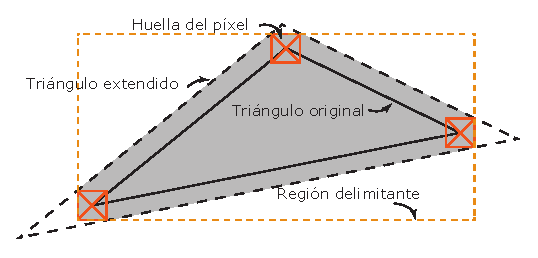
\includegraphics[width=0.7\linewidth]{media/conservative_triangle.eps}
	\caption{Polígono delimitante de un triángulo utilizado para rasterización conservativa.}
	\label{fig:expanded_bbpolygon}
\end{figure}

% subsection voxelizacion_conservativa (end)
% section voxelizacion (end)

\subsection{Composición de Fragmentos y Vóxeles}
\label{sub:frag_voxels}
Una vez que los fragmentos han sido generados en el \emph{fragment shader}, los valores deseados puede ser almacenados en una textura 3D utilizando operaciones de escritura que provee la extensión \emph{GL\_ARB\_shader\_image\_load\_store} en OpenGL \cite{ImageLoadStore}. Sin embargo múltiples fragmentos de diferentes triángulos puede caer sobre una misma posición en esta textura 3D. Bajo el ambiente paralelo del \emph{fragment shader} no es posible saber el orden en que los fragmentos son creados y procesados, esto se traduce en resultados arbitrarios cada vez que se revoxeliza la escena.

Para solventar este problema se utilizaron operaciones atómicas provistas por la misma extensión citada anteriormente. En nuestra implementación los valores necesarios a almacenar en vóxeles son normal, albedo y emisión. Una operación coherente y sencilla con respecto a estas propiedades en el espacio que envuelve un vóxel es un promedio.

\subsection{Voxelización Dinámica} % (fold)
\label{sub:voxelizacion_dinamica}
Para escenas complejas y densas en geometría poligonal el proceso de voxelización puede tomar considerable tiempo de ejecución afectando el rendimiento general del algoritmo si la escena necesita ser revoxelizada constantemente. Es por esto conveniente separar la voxelización de superficies estáticas y dinámicas en escena. La idea es voxelizar la parte estática de la escena una sola vez mientras que la parte dinámica es revoxelizada solo cuando sea necesario o constantemente por frame.

En nuestra implementación no se utiliza un \emph{octree} disperso para almacenar los vóxeles sino texturas 3D. La separación entre valores estáticos y dinámicos bajo el esquema de un \emph{octree} consiste en dividir el árbol en una parte dinámica y una parte estática. Considerando la cualidad dispersa de esta estructura esto no es de gran peso en memoria. 

Utilizando texturas 3D esto sería equivalente en nuestra implementación a generar en vez de tres texturas para almacenar albedo, normal y emisión se generarían seis. Tres de estas para la parte estática y tres para la parte dinámica. Esto es extremadamente ineficiente en memoria. Para evitar la creación de estas texturas se utiliza un volumen extra que permite indicar que vóxel forma parte de la parte estática y cuál no. Durante el proceso de voxelización dinámica solo los fragmentos que se encuentran dentro del espacio de un vóxel dinámico pueden escribir sobre la textura 3D.
% subsection voxelizacion_dinamica (end)

\section{Sombreado de Vóxeles} % (fold)
\label{sec:sombreado_de_voxeles}
Para el cálculo de iluminación indirecta es necesario sombrear cada vóxel. El proceso de sombreado de vóxeles nos permite almacenar la radiancia incidente sobre la escena discretizada en vóxeles. Utilizar mapas de luz-vista por cada fuente de luz como ya fue explicado en la sección \ref{subsub:voxel_capture}, puede ser ineficiente tanto en consumo de memoria como en rendimiento. Si se considera una escena con muchas luces, cada una de estas luces debe tener un mapa asociado y se debe repetir el proceso de captura por cada una de ellas. Otra desventaja de este método es la dependencia del rendimiento con la resolución del mapa de luz-vista. Al aumentar la resolución de esta textura también se aumenta el número de colisiones por cada fragmento que desea escribir sobre un mismo vóxel.

Nuestra implementación utiliza \emph{compute shaders} o el procesador de cómputo en la \ac{GPU} para el sombreado difuso de cada vóxel. Para calcular el término difuso sobre un fragmento utilizando la \ac{BRDF} de Lambert (ecuación \ref{eq:lambert}) se necesita saber el valor de $\rho_{d}$ el cual ya es almacenado en el volumen albedo. Esta constante luego debe ser multiplicada por el $\cos(N_{x}, \Psi)$ o atenuación normal. Por esto también se crea un volumen de normales. El vector $\Psi$ se obtiene a partir la dirección de cada fuente de luz en escena.

Para fuentes de luz con dirección no uniforme como luces puntuales o focales es además necesario saber la posición del fragmento a iluminar. Siendo cada vóxel una representación discreta de un espacio en escena, almacenado en una textura 3D, esta posición se extrae fácilmente convirtiendo la posición tridimensional del vóxel en espacio textura a su equivalente en espacio de mundo.

\begin{figure}[H]
	\centering
	\begin{subfigure}[t]{0.49\textwidth}
		\centering
		\captionsetup{justification=centering}
		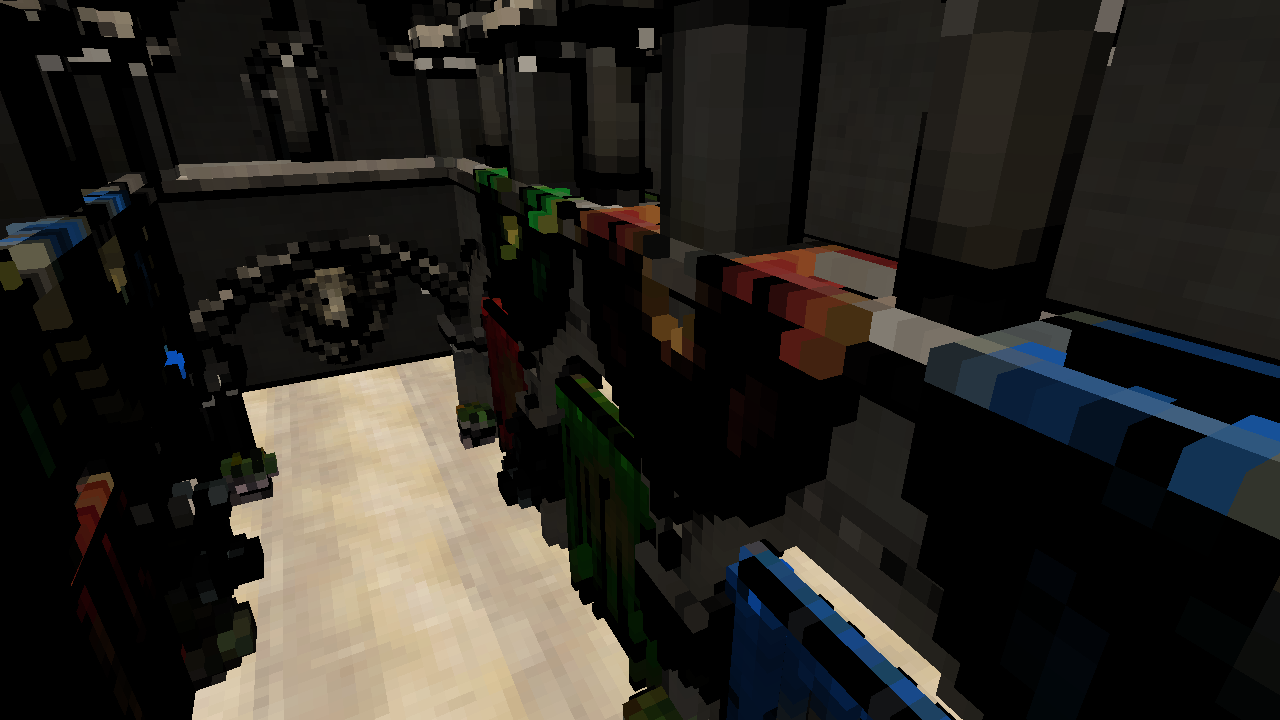
\includegraphics[width=\linewidth]{media/classic_lambert.png}
		\caption*{Lambert.}
	\end{subfigure}%
	\hspace{0.01\textwidth}
	\begin{subfigure}[t]{0.49\textwidth}
		\centering
		\captionsetup{justification=centering}
		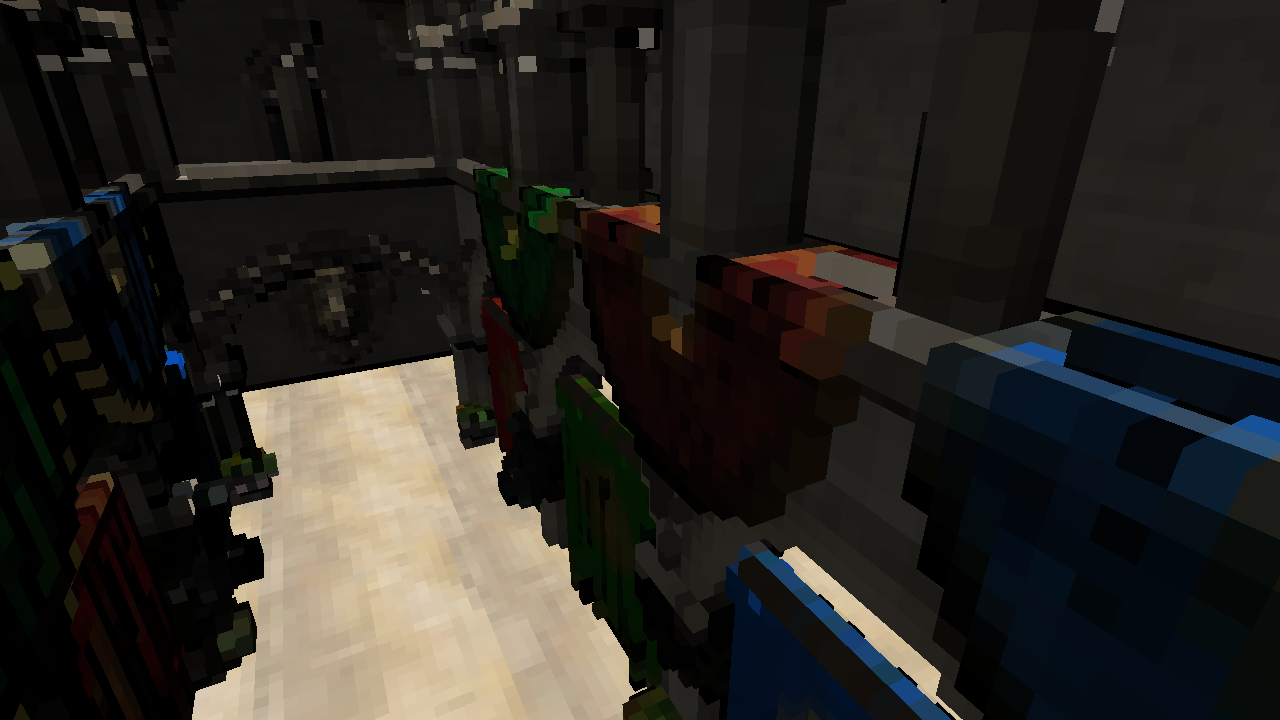
\includegraphics[width=\linewidth]{media/dir_lambert.png}
		\caption*{Lambert direccional ponderado.}
	\end{subfigure}%
	\caption{Sombreado difuso de vóxeles utilizando Lambert clásico y Lambert direccional ponderado.}
	\label{fig:lambert_dir_diff}
\end{figure}

Al promediar las normales en el espacio de un vóxel pueden surgir varios problemas de precisión. Esto sucede especialmente cuando un vóxel envuelve superficies finas cercanas con normales disparejas. Para disminuir este problema se implementaron dos modelos de iluminación de vóxeles: El modelo de Lambert clásico utilizando el vector normal promedio del vóxel directamente y otro denominado Lambert direccional ponderado, donde se calcula la atenuación normal por cada cara del vóxel, para promediar este resultado según el peso de cada eje en el vector normal promedio. En la Figura \ref{fig:lambert_dir_diff} se puede observar el sombreado resultante de ambos modelos. Para el segundo modelo algunos de los vóxeles totalmente negros recuperan parte de su color correcto y lugares sin disparidades en el vector normal, como el piso, mantienen el mismo color entre ambos modelos.
% section sombreado_de_voxeles (end)

\subsection{Trazado y Mapeo de Sombras sobre el Volumen} % (fold)
\label{sub:trazado_de_sombras_sobre_el_volumen}

Para obtener resultados coherentes durante el trazado de conos, es también necesario ocluir los vóxeles con sombras generadas a partir de distintas fuentes de luz en escena. En la Figura \ref{fig:voxel_shadow_error}, se puede observar iluminación excesiva en áreas ocluidas al no incluir sombras en la representación en vóxeles. Utilizando mapas de luz-vista como se explicó en la sección \ref{subsub:voxel_capture} esto es sencillo, ya que los vóxeles ocluidos simplemente no reciben fotones durante el proceso de captura de la iluminación directa.

\begin{figure}[H]
	\centering
	\begin{subfigure}[t]{0.49\textwidth}
		\centering
		\captionsetup{justification=centering}
		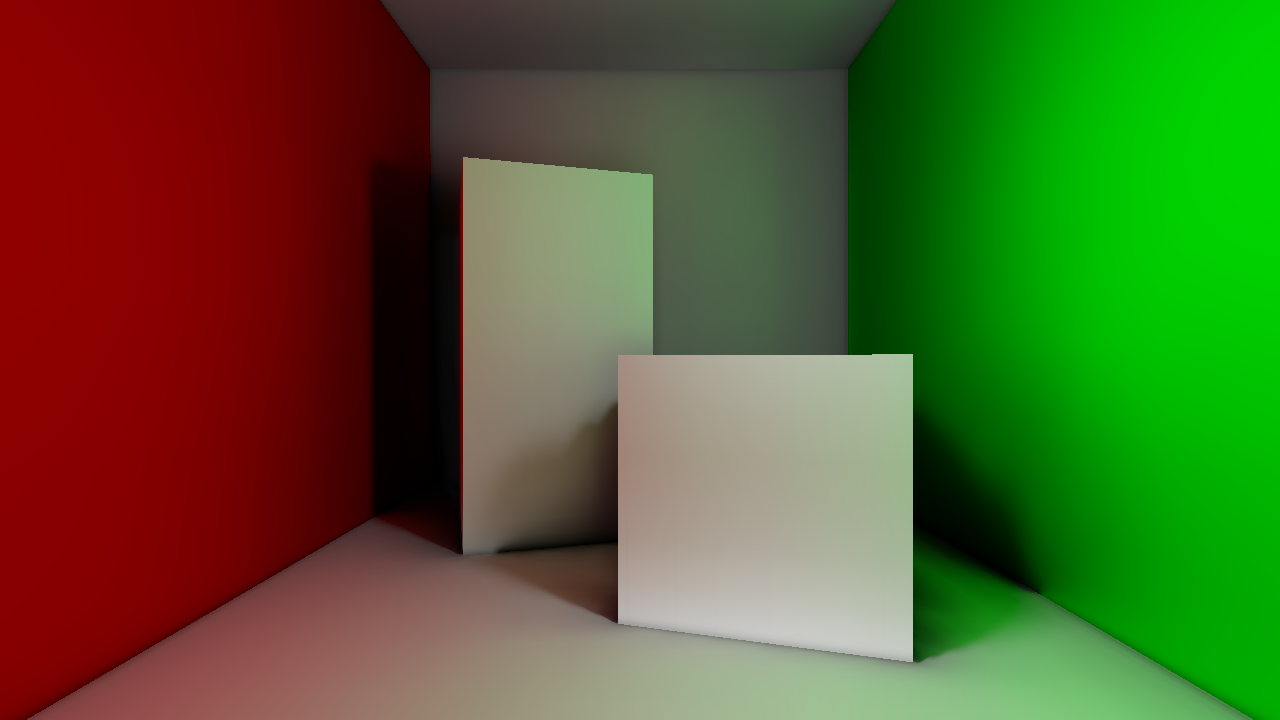
\includegraphics[width=\linewidth]{media/voxel_shadowing.png}
		\caption*{Con vóxeles ocluidos por sombras.}
	\end{subfigure}%
	\hspace{0.01\textwidth}
	\begin{subfigure}[t]{0.49\textwidth}
		\centering
		\captionsetup{justification=centering}
		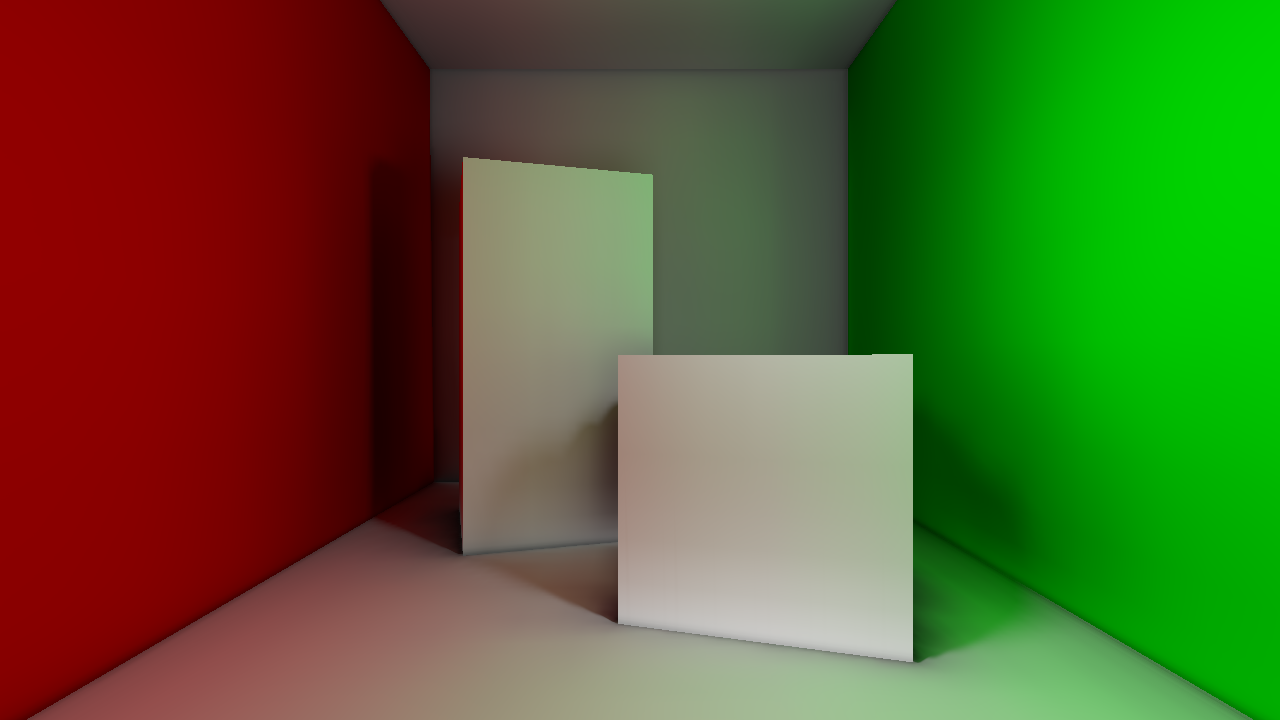
\includegraphics[width=\linewidth]{media/voxel_noshadowing.png}
		\caption*{Sin oclusión de vóxeles.}
	\end{subfigure}%
	\caption{Iluminación global al utilizar una representación con vóxeles sin y con oclusión por sombras.}
	\label{fig:voxel_shadow_error}
\end{figure}

En nuestra implementación existen distintas opciones para trazar sobras sobre los vóxeles. Este proceso se realiza durante el sombreado de vóxeles explicado anteriormente. 

Para luces directas se utiliza mapeo de sombras visto en la sección \ref{subsec:shadowmapping}. En esta técnica es necesario obtener la posición en espacio de mundo del vóxel. Para esto la posición tridimensional del vóxel en espacio de textura se transforma a espacio de mundo. De la transformación se obtiene la posición central del vóxel. Utilizar el centro del vóxel para mapeo de sombras, puede ocasionar problemas cuando este punto esta ocluido por otras superficies dentro del mismo vóxel o fragmentos cercanos (ver Figura \ref{fig:voxel_shadow_translate}). Esto sucede ya que el mapa de sombras es una representación mucho más detallada de la escena vista desde una fuente de luz. Para solventar este problema se traslada la posición del vóxel según el vector normal por el tamaño medio de un vóxel.

\begin{figure}[H]
	\centering
	\begin{subfigure}[t]{0.49\textwidth}
		\centering
		\captionsetup{justification=centering}
		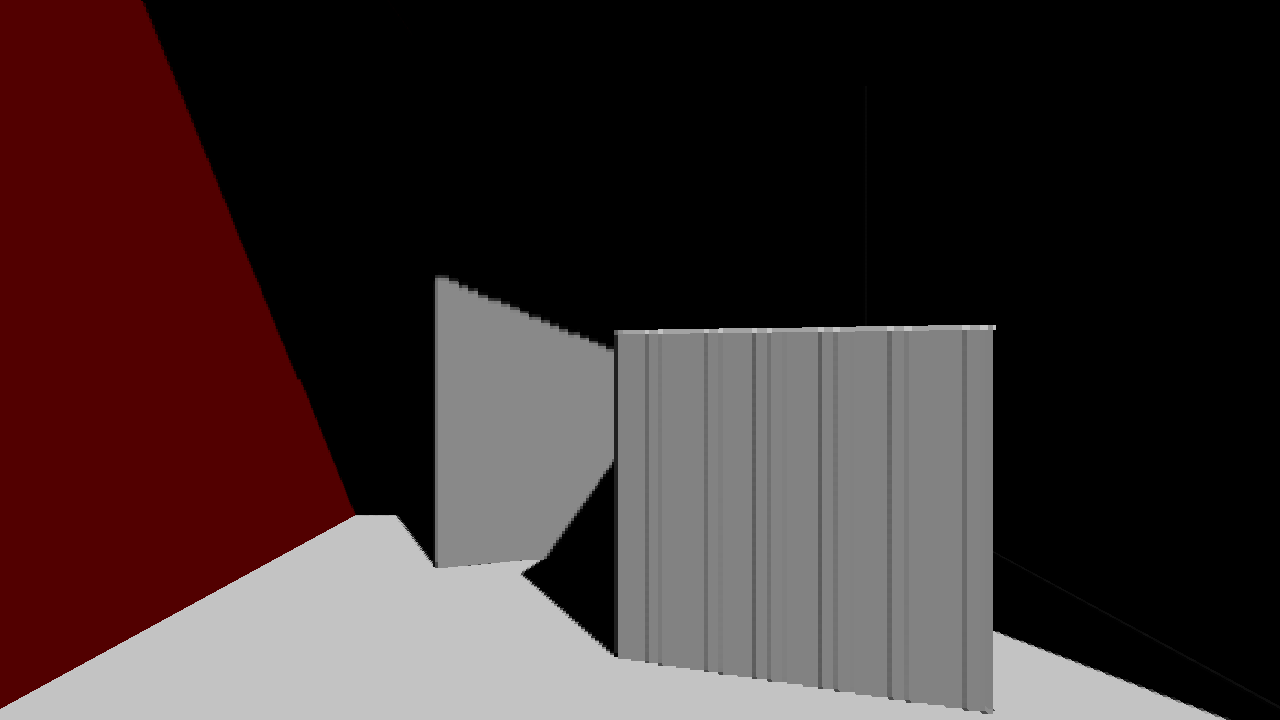
\includegraphics[width=\linewidth]{media/no_translation.png}
		\caption*{Utilizando la posición del centro del vóxel.}
	\end{subfigure}%
	\hspace{0.01\textwidth}
	\begin{subfigure}[t]{0.49\textwidth}
		\centering
		\captionsetup{justification=centering}
		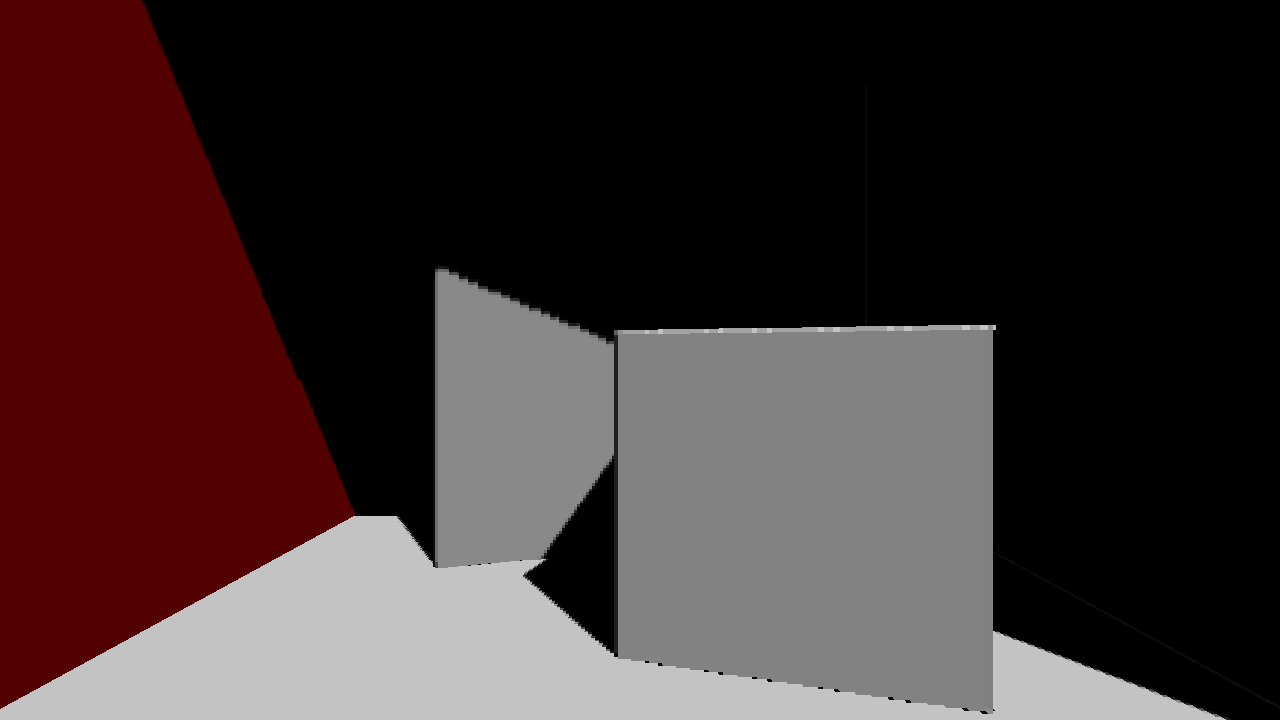
\includegraphics[width=\linewidth]{media/with_translation.png}
		\caption*{Trasladando la posición medio vóxel.}
	\end{subfigure}%
	\caption{Sombras sobre vóxeles con y sin traslado de la posición de sombreado.}
	\label{fig:voxel_shadow_translate}
\end{figure}

Estando el mapeo de sombras disponible en nuestra implementación para solo una luz directa, se implementó trazado de sombras para cualquier fuente de luz puntual, focal o direccional. Los volúmenes resultantes del proceso de voxelización pueden ser utilizados para trazar rayos sobre la escena discretizada. Siendo estos volúmenes una representación mucho más simple de la escena original, utilizar técnicas de comunes en trazado de rayos (sección \ref{subsec:monte_carlo_raytracing}) es viable.

Para realizar pruebas de oclusión sobre un vóxel por una fuente de luz, se lanza un rayo desde la posición del vóxel en la dirección opuesta de la luz incidente. Si este rayo colisiona con otro vóxel entonces el de origen está ocluido.

\subsubsection{Trazado de Sombras Suaves sobre el Volumen}

Una técnica que incrementa la calidad visual de las sombras es la generación de un bordeado suave para las sombras. En trazado de rayos esto se logra lanzando varios rayos en distintas direcciones a diferencia de uno solo para generar varias muestras de oclusión.

En nuestra implementación se logra obtener bordes suaves para las sombras generadas durante el sombreado de vóxeles con un solo rayo. Esta técnica se fundamenta en el hecho de que al trazar un rayo hacia una superficie voxelizada, este rayo colisionara más veces contra vóxeles cerca de los bordes de la superficie vistos desde la fuente de luz. Como se observa en la Figura \ref{fig:soft_voxel_shadow}, en vez de detener el rayo una vez que se ha encontrado una colisión, ahora se le asigna un valor a cada colisión y se va acumulando este factor a través del recorrido del rayo dividido por la distancia recorrida.

\begin{figure}[H]
	\centering
	\begin{subfigure}[t]{0.49\textwidth}
		\centering
		\captionsetup{justification=centering}
		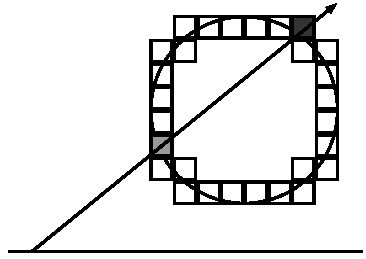
\includegraphics[width=\linewidth]{media/shadow_tracer.pdf}
		\caption*{Rayo alejado de los bordes de la superficie.}
	\end{subfigure}%
	\hspace{0.01\textwidth}
	\begin{subfigure}[t]{0.49\textwidth}
		\centering
		\captionsetup{justification=centering}
		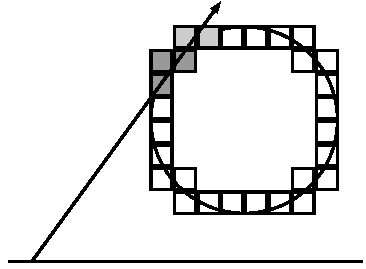
\includegraphics[width=\linewidth]{media/shadow_trace_corner.pdf}
		\caption*{Rayo cercano al el borde de la superficie.}
	\end{subfigure}%
	\caption{Descripción gráfica del proceso de acumulación de colisiones a través del recorrido de un rayo para prueba de oclusión.}
	\label{fig:soft_voxel_shadow}
\end{figure}

% subsection trazado_de_sombras_sobre_el_volumen (end)

\section{Representacion en Voxeles}
\section{Trazado de Conos con Vóxeles} % (fold)

\label{sec:trazado_de_conos_con_voxeles}

El proceso de trazado de conos con vóxeles funciona de manera similar a marcha de rayos o \emph{ray-marching}. La diferencia es que el volumen a muestrear por cada paso que da el rayo incrementa según la distancia al punto de origen del cono (ver Figura \ref{fig:vct_explain}). La forma del cono es esencialmente una discretización de un grupo de rayos trazados desde un punto en una superficie. Para obtener las muestras de volúmenes cada vez más grande se utilizan los niveles de \emph{mipmap} en la estructura de vóxeles.

\begin{wrapfigure}{l}{0.4\linewidth}
	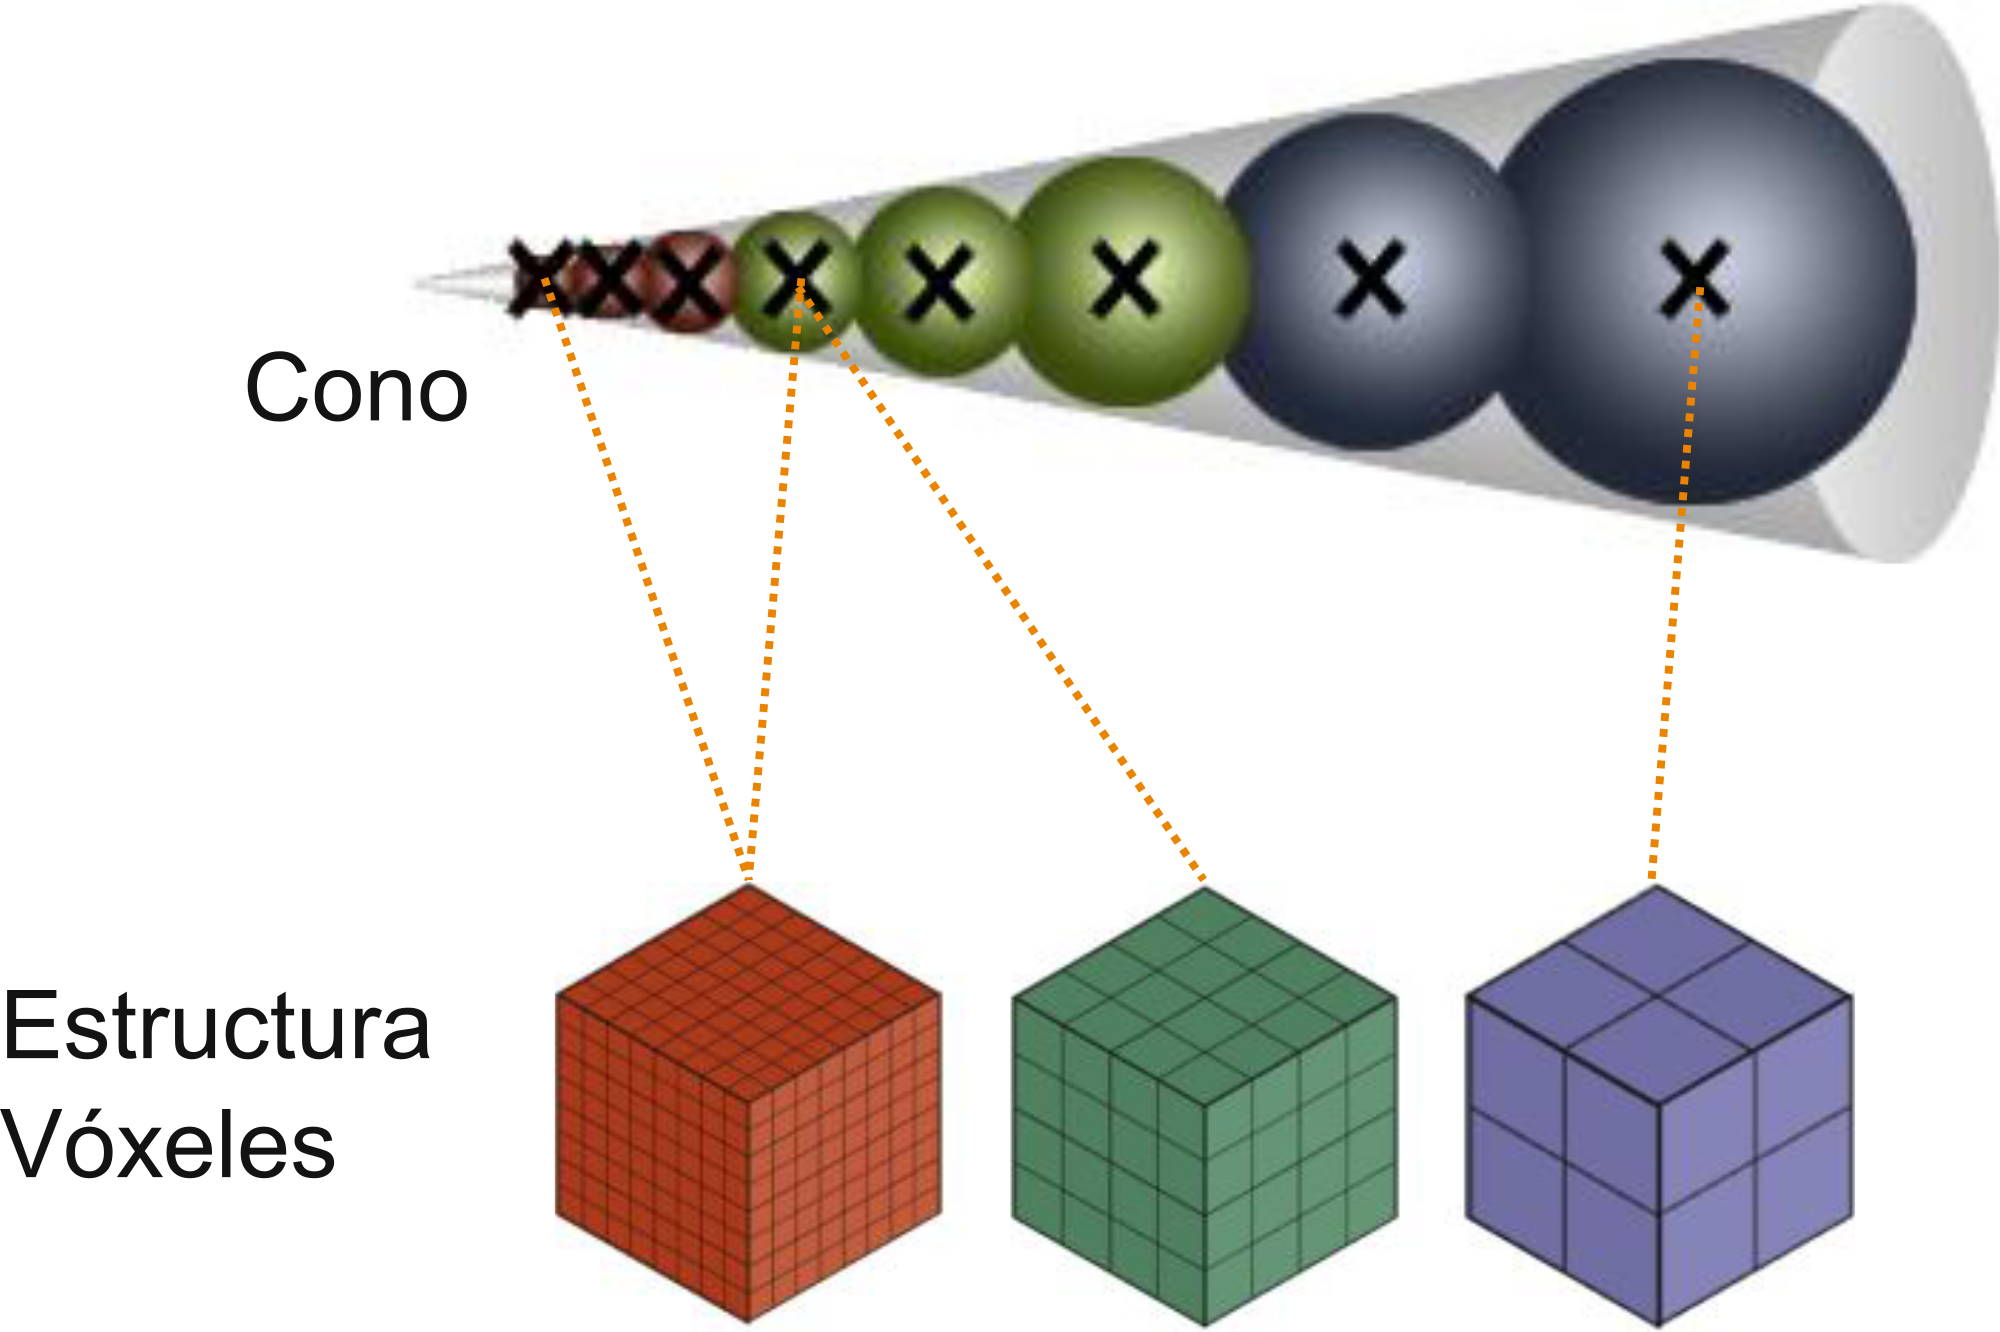
\includegraphics[width=0.95\linewidth]{media/vct_explain.png}
	\caption{Descripción gráfica del trazado de conos con vóxeles e interpolación entre distintos niveles de detalle \cite{Oliver:2012:UEE:2341836.2341909}.}
	\label{fig:vct_explain}
\end{wrapfigure}

\noindent Nuestra implementación realiza trazado de conos con vóxeles de la misma manera que fue explicada en la sección \ref{sub:voxel_cone_tracing_orig}, ya mayor diferencia reside en el uso de texturas 3D. Una de las principales ventajas de utilizar texturas 3D es que estas aceleran considerablemente el muestreo de la estructura jerárquica de vóxeles. Mientras que con un \emph{octree} cada vez que se desea trazar un cono el árbol tiene que ser recorrido de forma recursiva. Con texturas 3D esto se reduce a una simple instrucción proveída por OpenGL llamada \emph{textureLod}. Esta función recibe una textura, una coordenada de muestreo y un nivel de \emph{mipmap}. La función también realiza interpolación lineal entre los distintos niveles de \emph{mipmapping} si la textura a muestrear así lo habilita.
% section trazado_de_conos_con_voxeles (end)
\subsection{Reflexión Difusa}
La reflexión difusa de un fragmento puede ser aproximada utilizando integración Monte Carlo, trazando un número de conos sobre la semiesfera orientada por el vector normal del fragmento, y acumulando la radiancia a través del recorrido del cono. En nuestra implementación se utilizan seis conos difusos distribuidos de forma uniforme sobre la semiesfera (ver Figura \ref{fig:brdf_cones2}) orientada por el vector normal del fragmento.
\subsection{Oclusión Ambiental}
\label{sub:occl_ambt_prop}
La oclusión ambiental sobre un fragmento puede ser aproximada trazando conos sobre la semiesfera orientada por el vector normal de este. Para la oclusión ambiental solo es relevante acumular información de oclusión. El cono ambiental es ponderado por una función $f(r)$ donde su valor decae según la distancia recorrida. En nuestra aplicación se utiliza la función:
\begin{equation}
	f(r) = \frac{1}{1+\lambda r}
\end{equation} donde $r$ representa el radio del cono y $\lambda$ una variable personalizada que describe la intensidad de declive según la distancia para el término de oclusión ambiental, básicamente la extensión del radio de oclusión.
\subsection{Reflexión Especular}
Nuestra implementación utiliza como modelo de iluminación la \ac{BRDF} Blinn-Phong. Para obtener la reflexión especular es necesario solo un cono en equivalencia al lóbulo especular de la \ac{BRDF} como se observa en la Figura \ref{fig:brdf_cones2}. La apertura del cono especular depende del factor $n$ en Blinn-Phong, mientras más alto es este valor menor es la apertura del cono especular.
\begin{figure}[H]
	\centering
	\begin{subfigure}[t]{.32\linewidth}
		\centering
		\captionsetup{justification=centering}
		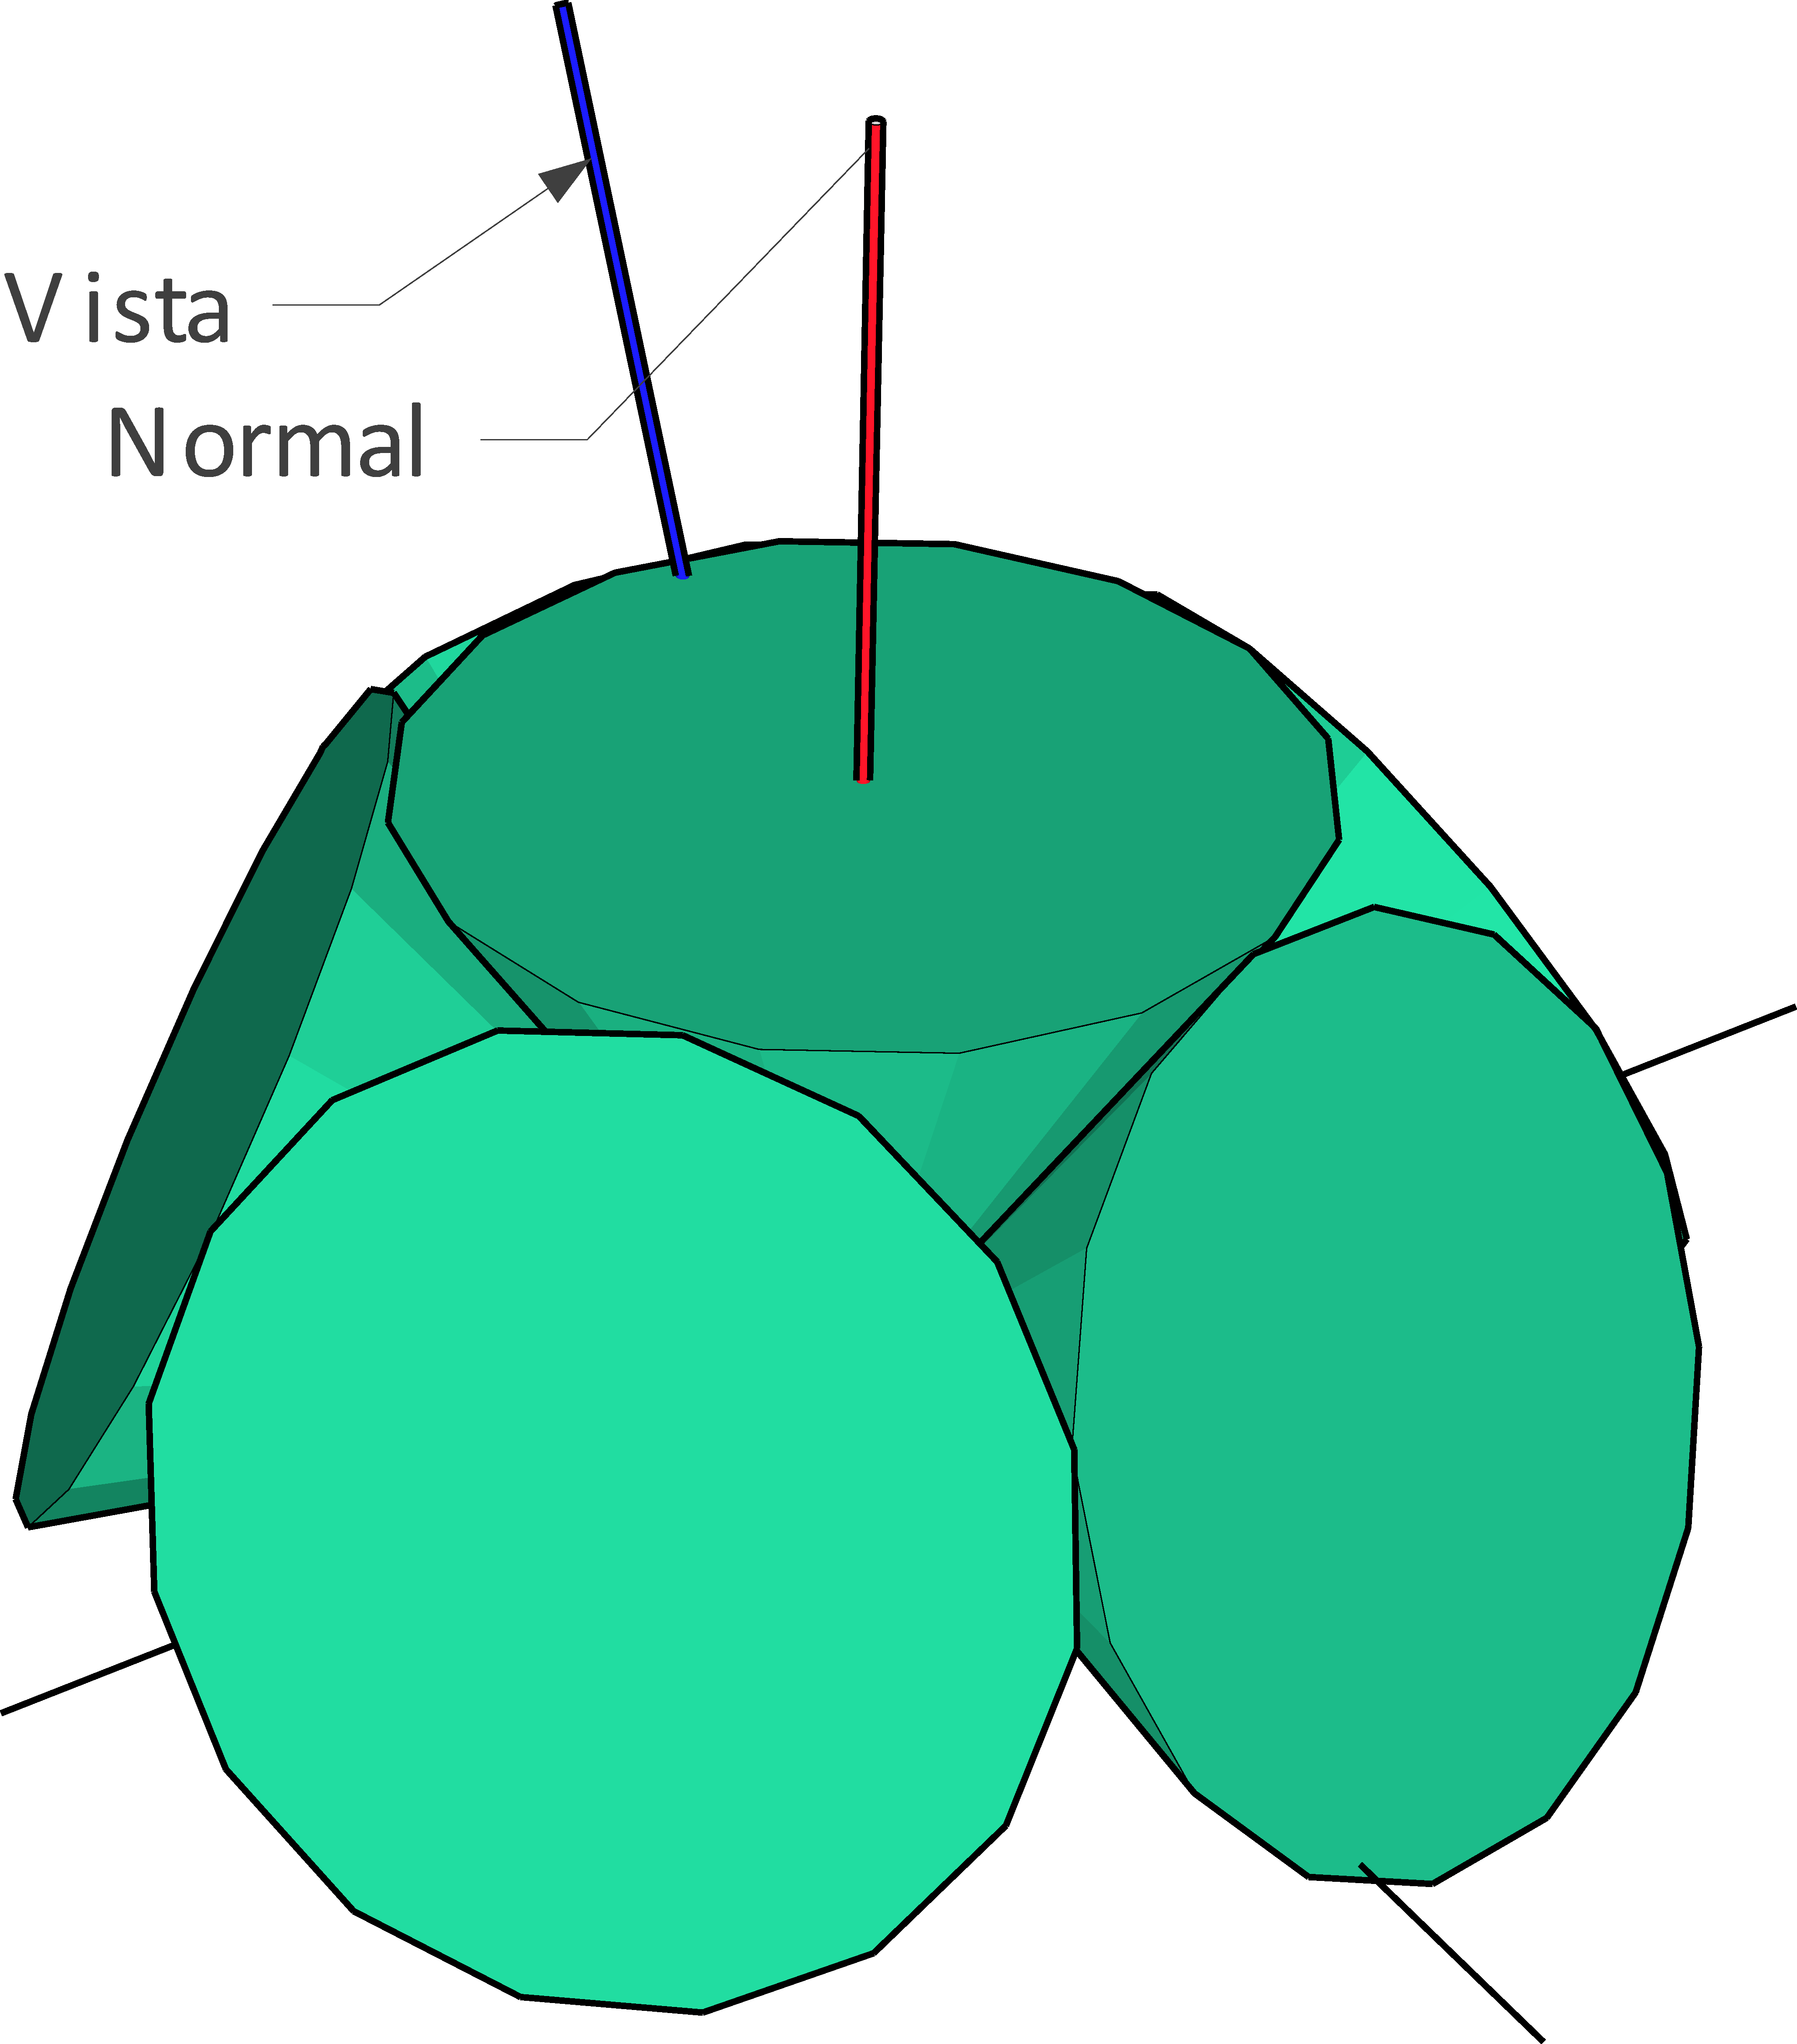
\includegraphics[width=\linewidth]{media/diffuse_cones_cropped.pdf}
		\caption*{Conos sobre la semiesfera para reflexión difusa.}
	\end{subfigure}%
	\hspace{0.01\textwidth}
	\begin{subfigure}[t]{.32\linewidth}
		\centering
		\captionsetup{justification=centering}
		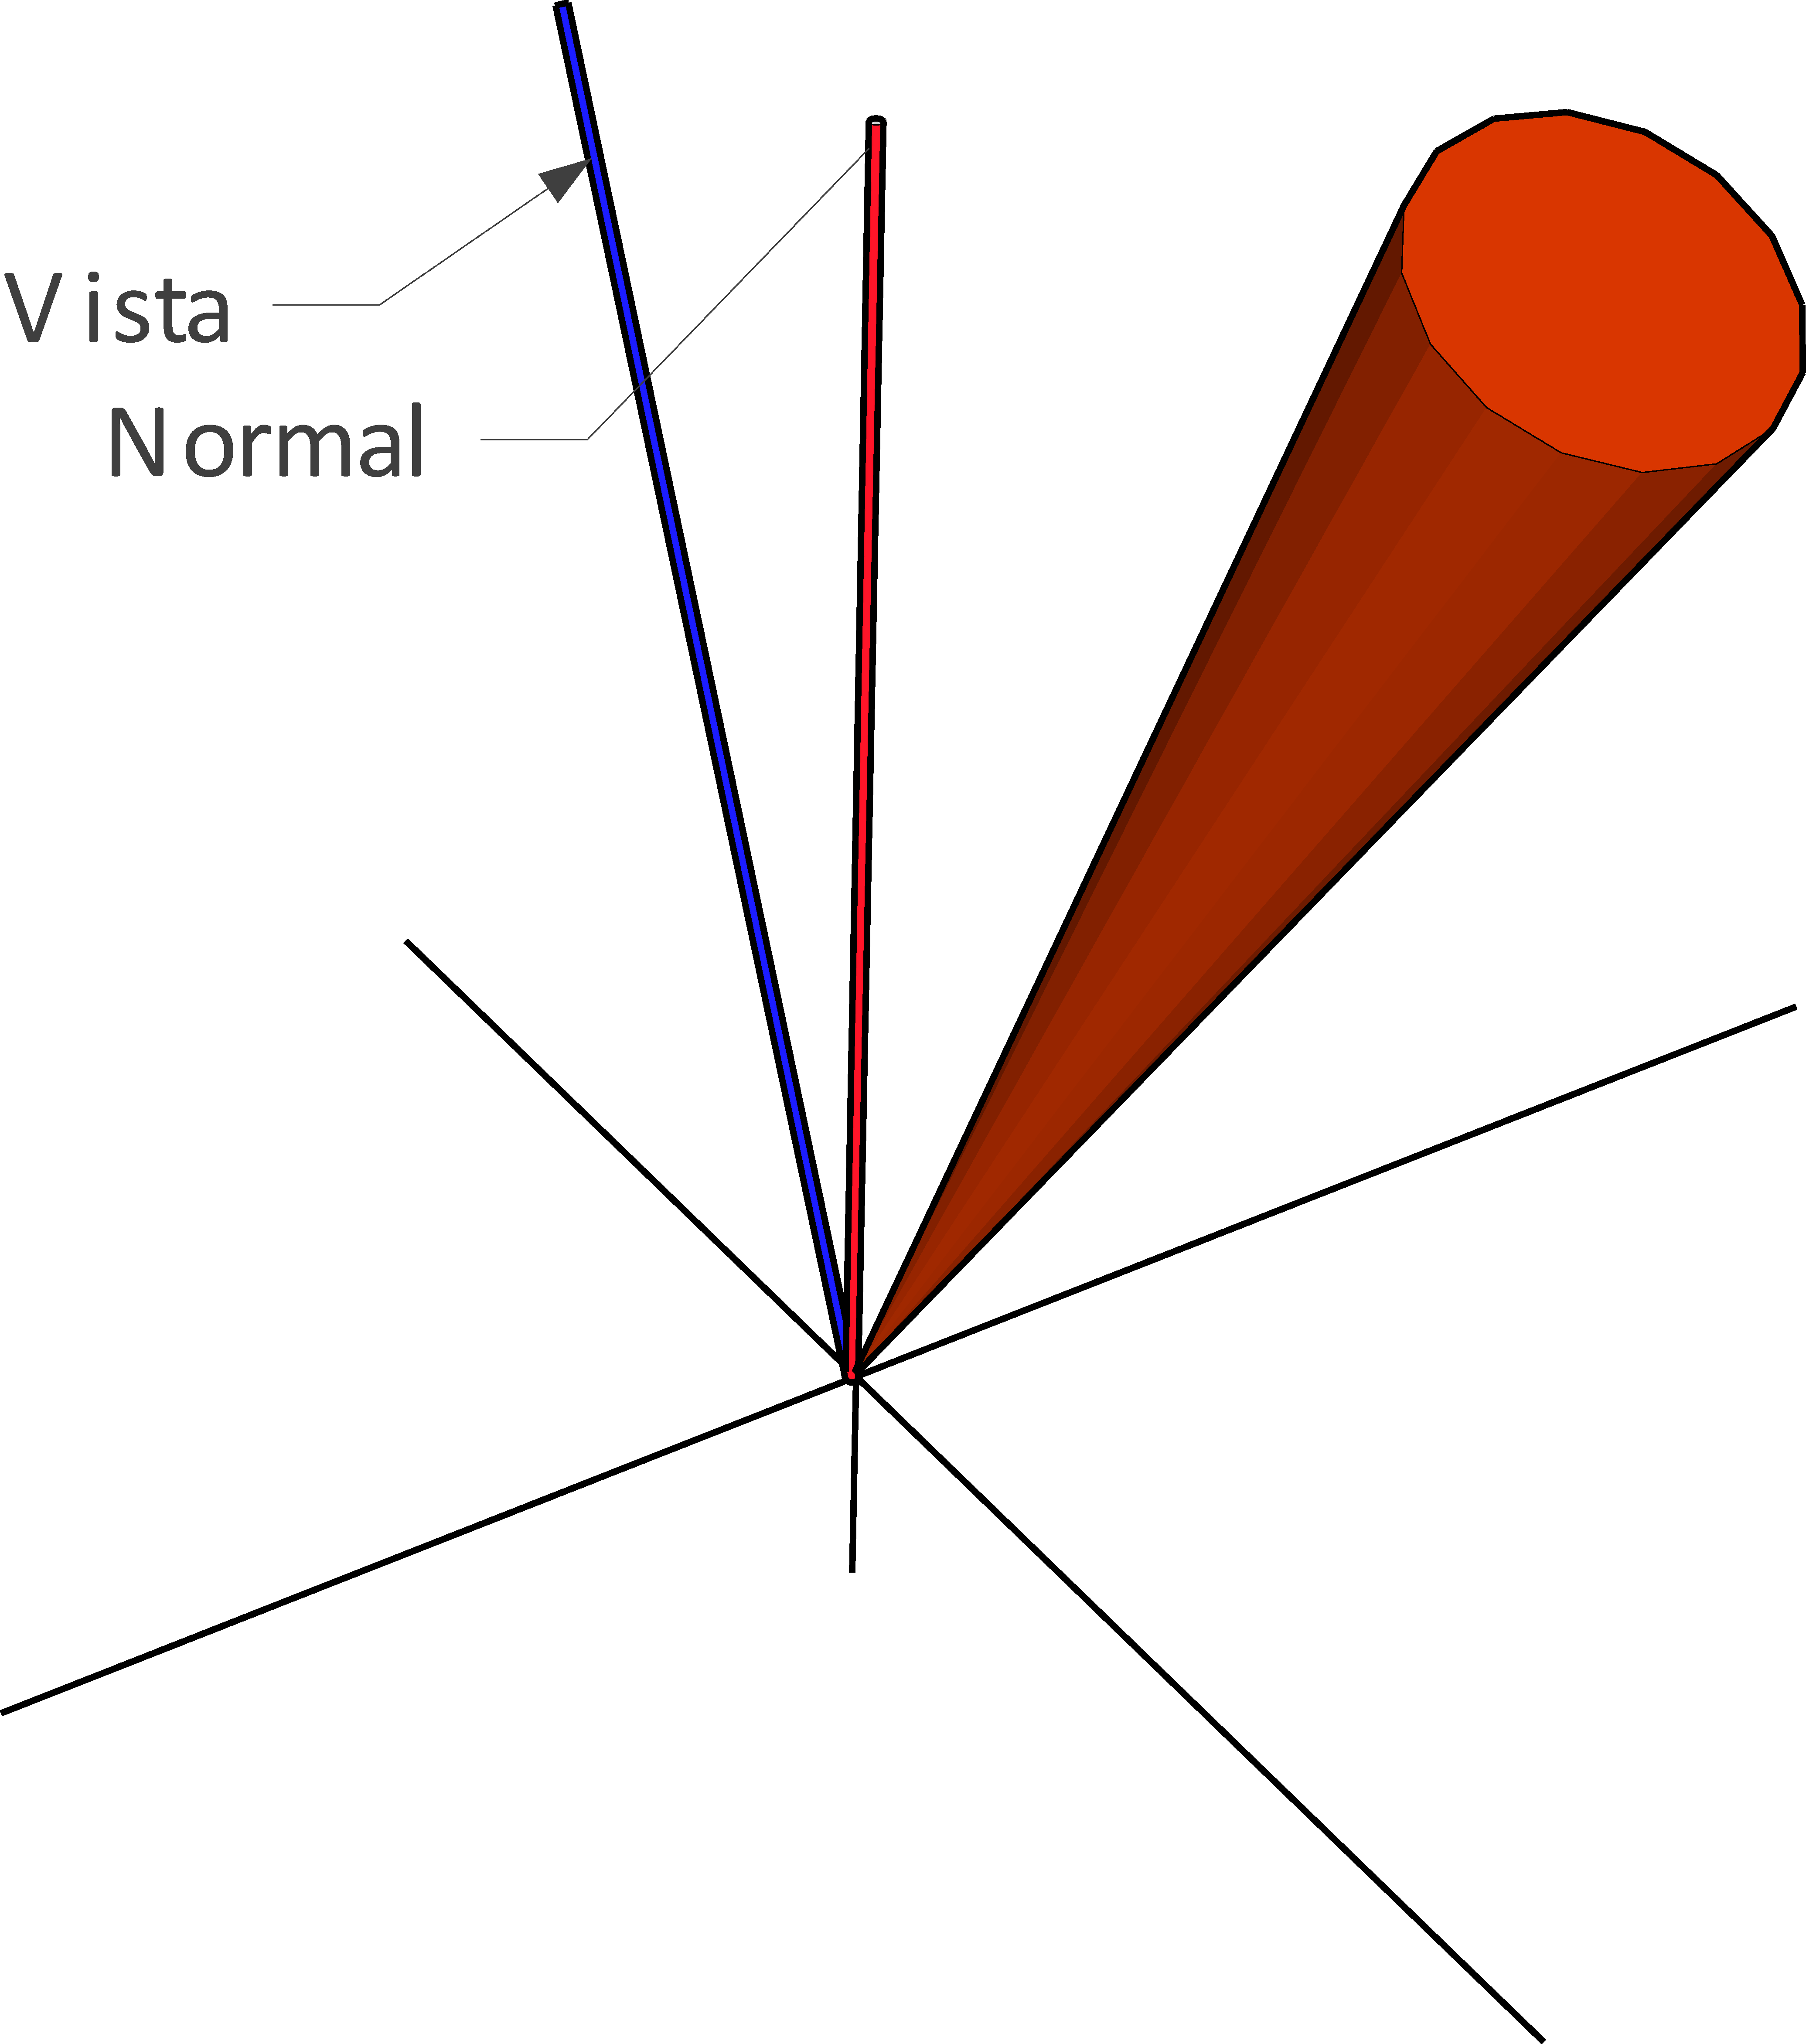
\includegraphics[width=\linewidth]{media/specular_cone_cropped.pdf}
		\caption*{Cono para el lóbulo especular.}
	\end{subfigure}%
	\hspace{0.01\textwidth}
	\begin{subfigure}[t]{.32\linewidth}
		\centering
		\captionsetup{justification=centering}
		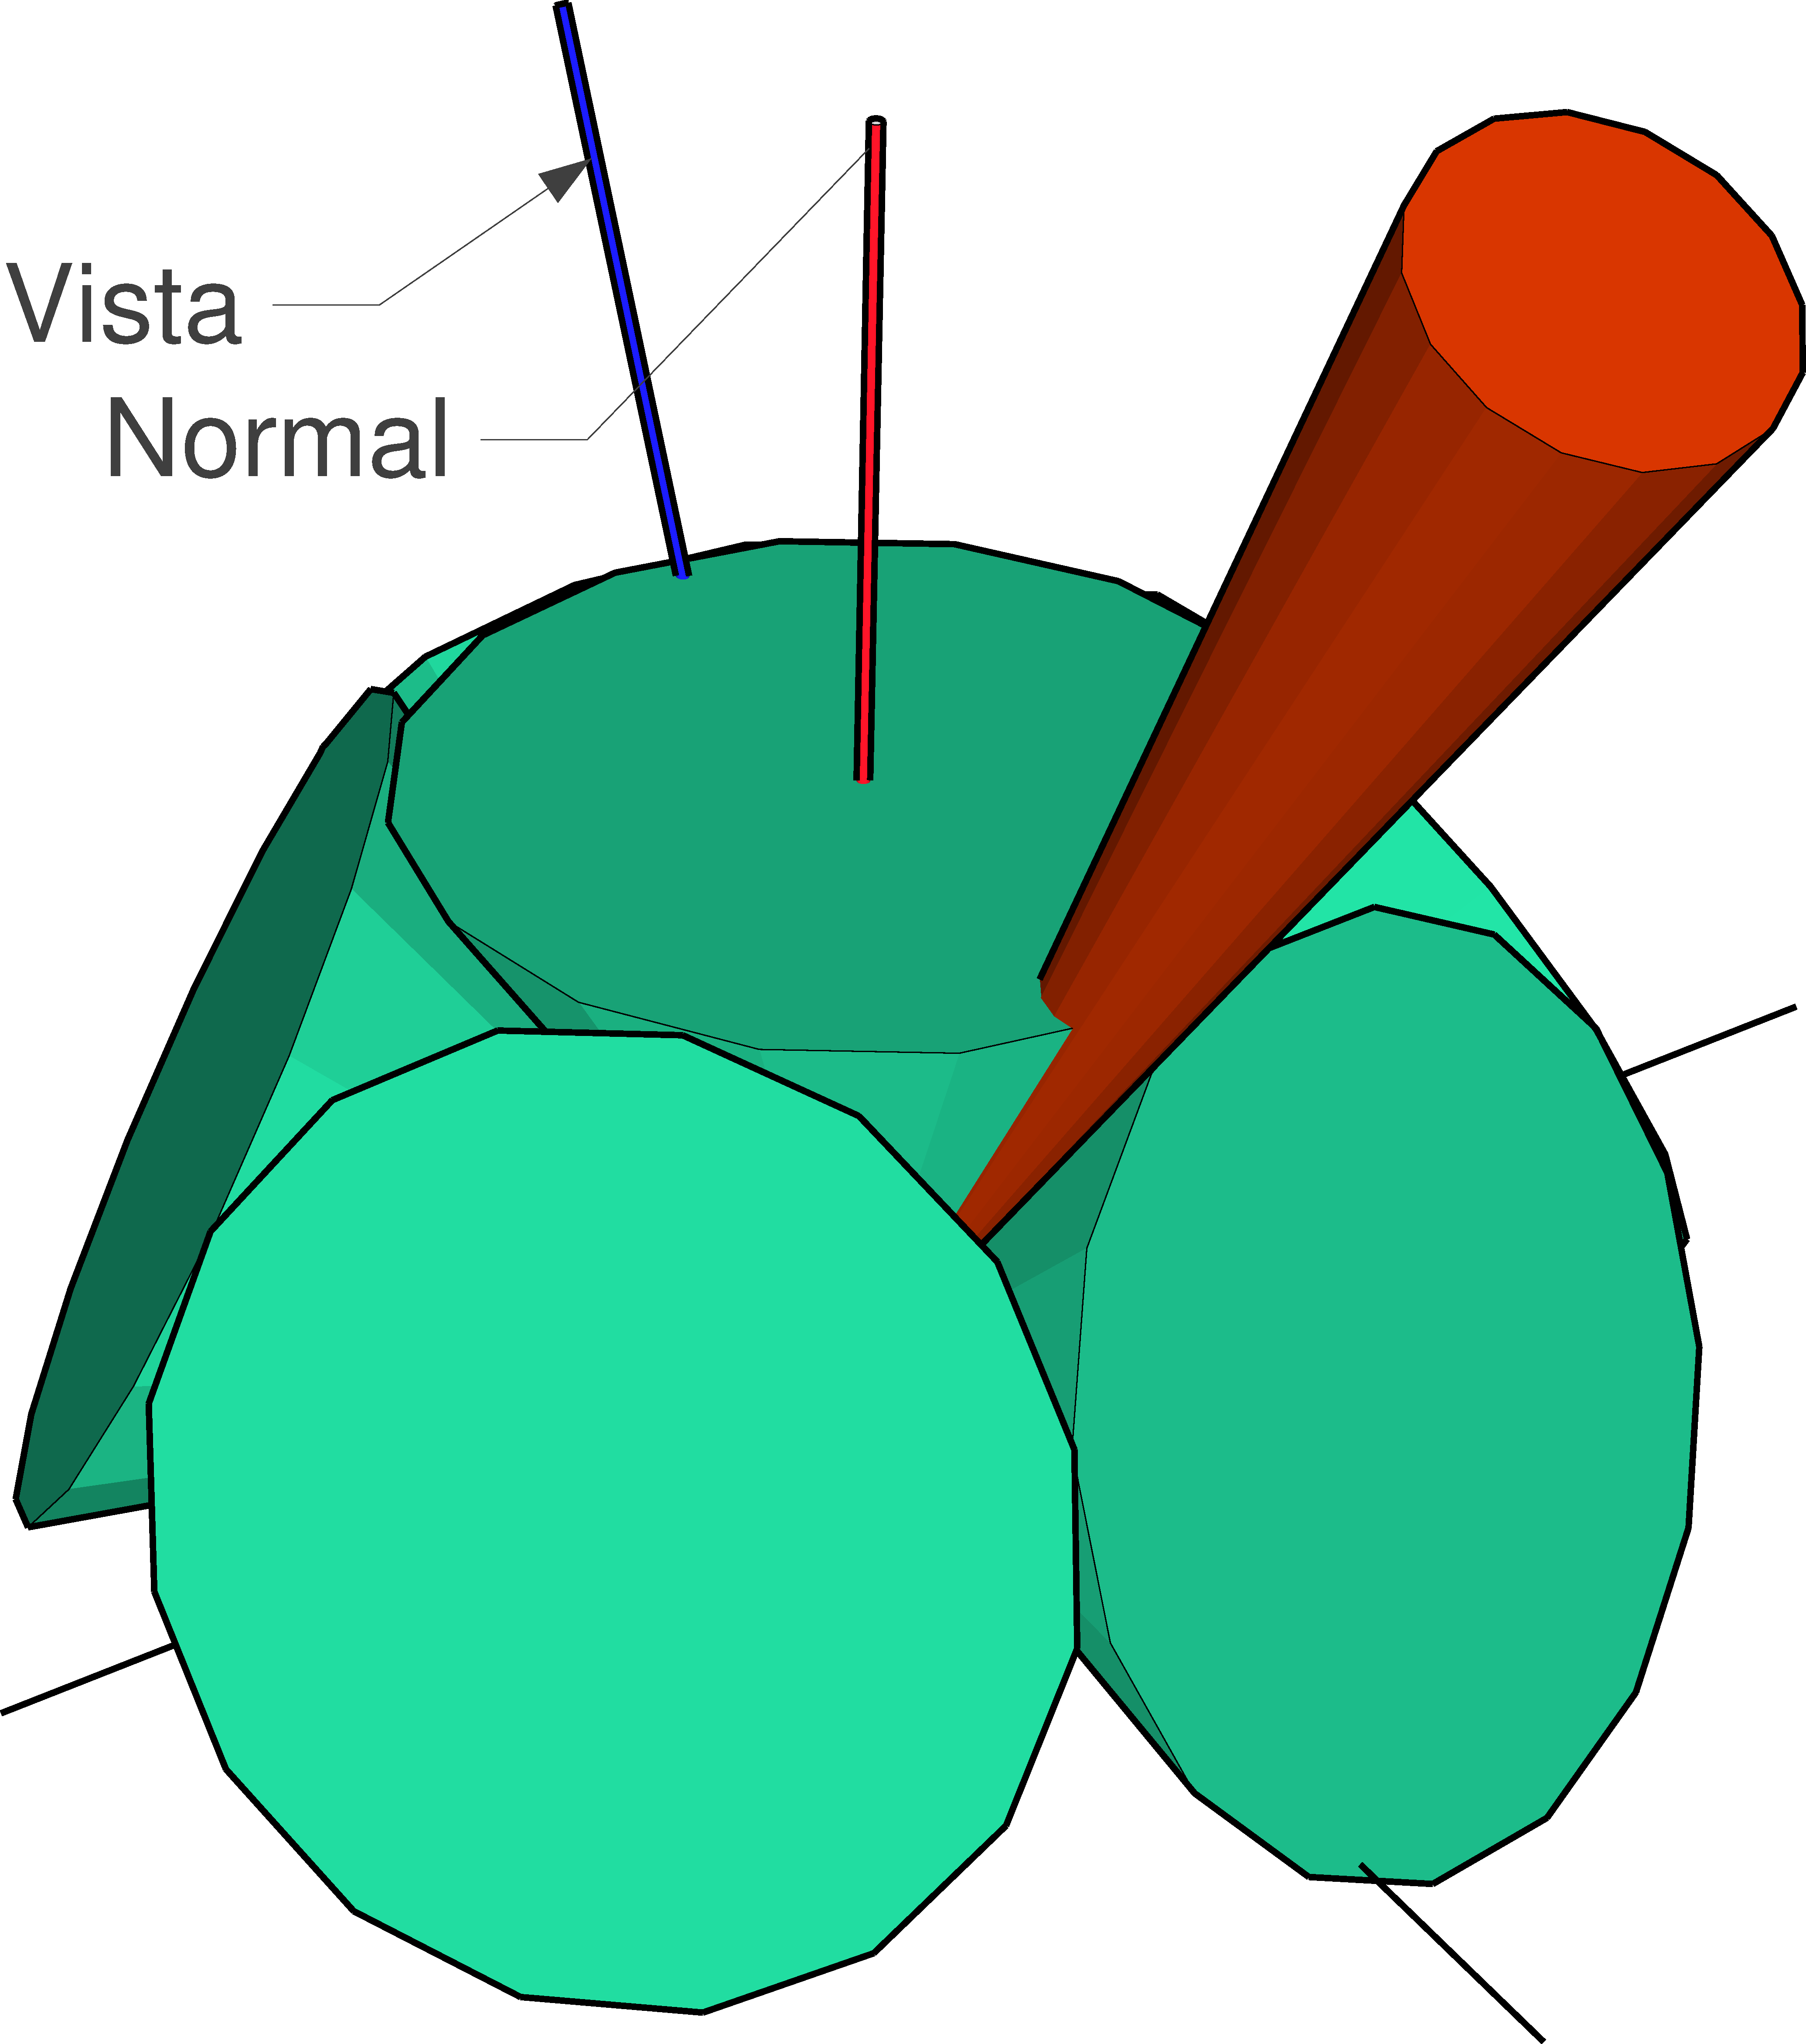
\includegraphics[width=\linewidth]{media/brdf_cones_cropped.pdf}
		\caption*{Discretización de la BRDF en conos.}
	\end{subfigure}%
	\caption{Ilustración de la distribución de los conos utilizados para representar la \ac{BRDF} Blinn-Phong.}
	\label{fig:brdf_cones2}
\end{figure}

\subsection{Sombras Suaves} % (fold)
\label{sub:sombras_suaves_con_trazado_de_conos}
El trazado de conos contra vóxeles también puede ser utilizado para realizar pruebas de oclusión sobre una superficie. En nuestra implementación se traza un cono desde la posición del fragmento en dirección opuesta a la dirección de la luz incidente. Para este cono se acumula la opacidad de los vóxeles. La apertura del cono permite controlar el umbral de la sombra resultante. A mayor apertura más suave y esparcida es la sombra. En la Figura \ref{fig:shadow_cone_prop} se describe el trazado de este cono.

\begin{figure}[H]
	\centering
	\captionsetup{justification=centering}
	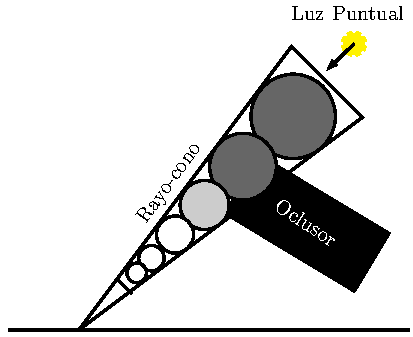
\includegraphics[width=.4\linewidth]{media/shadow_cone.pdf}
	\caption{Descripción gráfica del recorrido de un cono empleado para sombreado de superficies.}
	\label{fig:shadow_cone_prop}
\end{figure}

% subsection sombras_suaves_con_trazado_de_conos (end)

\section{Iluminación Global de Vóxeles} % (fold)
\label{sec:iluminacion_global_de_voxeles}
Almacenando solo la radiancia producto de la iluminación directa nos permite obtener iluminación indirecta de un solo rebote durante el proceso de trazado de conos con vóxeles. Esto provee buenos resultados visuales ya que el primer rebote es usualmente el que más contribuye en el transporte de luz de una escena.

Para la incorporación de un segundo rebote nuestra implementación realiza trazado de conos con vóxeles dentro de la misma representación con vóxeles utilizando compute shaders. 

Luego que el proceso de sombreado de vóxeles es completado y se filtran estos valores para generar vóxeles anisótropos, se agrega otro pasó para calcular el primer rebote de iluminación global sobre el volumen de radiancia. Similar al trazado de conos por fragmento explicado en \ref{sub:voxel_cone_tracing_orig} ahora por cada vóxel se trazan conos acumulando la radiancia incidente sobre el vóxel. Este método solo comprende reflexión difusa ya que en nuestra implementación no se almacena información especular durante el proceso de voxelización. Al finalizar de calcular la iluminación global sobre cada vóxel se vuelve a realizar el filtrado anisótropo. El volumen resultante ahora es utilizado durante la composición final de la imagen por el trazado de conos con vóxeles, donde ahora estos conos acumulan radiancia producto de tanto iluminación directa como indirecta difusa.
% section iluminacion_global_de_voxeles (end)

\section{Materiales Emisivos} % (fold)
\label{sec:materiales_emisivos}
La estructura de vóxeles utilizada durante el trazado de conos almacena un valor de radiancia por cada vóxel. Considerando esto, agregar materiales emisivos al proceso de voxelización es simple. Para la voxelización de materiales emisivos se utiliza otro volumen además de los ya existentes (albedo y normal) durante el proceso de voxelización. Este volumen almacenaría el promedio de emisión de los fragmentos que envuelve el vóxel. El valor de estos vóxeles es luego agregado al cálculo de radiancia directa durante el proceso de sombreado de vóxeles. Los materiales emisivos pueden ser utilizados para aproximar cualquier clase de superficie luminosa como luces de área.
% section materiales_emisivos (end)

